% Created 2024-10-05 Sat 21:30
% Intended LaTeX compiler: pdflatex
\documentclass[12pt]{article}
\usepackage[utf8]{inputenc}
\usepackage[T1]{fontenc}
\usepackage{graphicx}
\usepackage{longtable}
\usepackage{wrapfig}
\usepackage{rotating}
\usepackage[normalem]{ulem}
\usepackage{amsmath}
\usepackage{amssymb}
\usepackage{capt-of}
\usepackage{hyperref}
\usepackage[margin=1in]{geometry} \usepackage{amsmath} \usepackage{svg}
\author{Jason Press}
\date{}
\title{Breaking Fishing Line}
\hypersetup{
 pdfauthor={Jason Press},
 pdftitle={Breaking Fishing Line},
 pdfkeywords={},
 pdfsubject={},
 pdfcreator={Emacs 29.4 (Org mode 9.7.11)}, 
 pdflang={English}}
\begin{document}

\maketitle
\section{Introduction}
\label{sec:orgcb4995c}

In this lab, we added an increasing amount of mass to a mass hanger suspended by two fishing lines, one rated for four pounds of force and the other rated for eight pounds of force. The goal of the lab was to predict which line would break first. To obtain the maximum amount of tension each line can handle, we added an increasing amount of mass to a mass hanger suspended by one line until the line broke. The amount of mass that the string held before it broke is the maximum amount of weight \(m\) it can hold, so the amount of tension the line can handle is \(mg\).

In the setup, let \(m_1\) be the line of choice, \(\theta_1\) be the angle that line \(m_1\) makes from the mounting point, \(M_1\) be the maximum amount of tension that \(m_1\) can handle, and \(\theta\)\textsubscript{2} be the angle that the other line makes from the mounting point. For a visual depiction, see Figure \ref{fig:setup}. Using Newton's Second Law gives the maximum amount of weight \(m_1\) can handle before snapping in the experimental setup:

\begin{align}\label{eq:tension}
m_{1} = M_{1} \left( \sin\theta_1 + \cos\theta_1\tan\theta_2 \right)
\end{align}

The amount of weight \(m_2\) can handle also uses Equation \ref{eq:tension}, with \((1,2 := 2,1)\). The maximum amount of weight that the experimental setup can handle is therefore \(\min(m_{1}, m_{2})\).

To calculate error, we used the following equation:

\begin{equation}
\begin{aligned} \label{eq:error}
\sigma_{m_1}^2 = \left[ \sin\theta_1 + \cos\theta_2\tan\theta_2 \right]^2\sigma_{M_1}^2 \\
+ \left[ M_1 \left( \cos\theta_1 - \sin\theta_1\tan\theta_2 \right) \right]^2 \sigma_{\theta_1}^2 \\
+ \left[ M_1 \left( \sin\theta_1 + \cos\theta_1\sec^2\theta_2 \right) \right]^2 \sigma_{\theta_2}^{2}
\end{aligned}
\end{equation}

The equation for \(\sigma_{m_2}^2\) follows naturally.
\section{Methods}
\label{sec:org5aca3eb}

This lab has two components: the experimental setup, with the hanging mass suspended by two fishing lines; and testing each line for tension.

Additionally, we tied each line with a double cinch knot followed by half hitches for the remaining tail of the line. This ensured the system did not fall because a knot slipped.
\subsection{The Experimental Setup}
\label{sec:org79b9add}

For the experimental setup, we tied both lines to the ceiling on two convenient locations, some arbitrary distance apart. Then, we tied each line to the mass hanger, labeled \texttt{w} in Figure \ref{fig:setup}. After predicting the result, we tested the prediction by placing more and more mass on the mass hanger until one line snapped, causing the whole setup to fall to the ground (the second line snapped after the first due to the lack of support from the first line).

\begin{center}
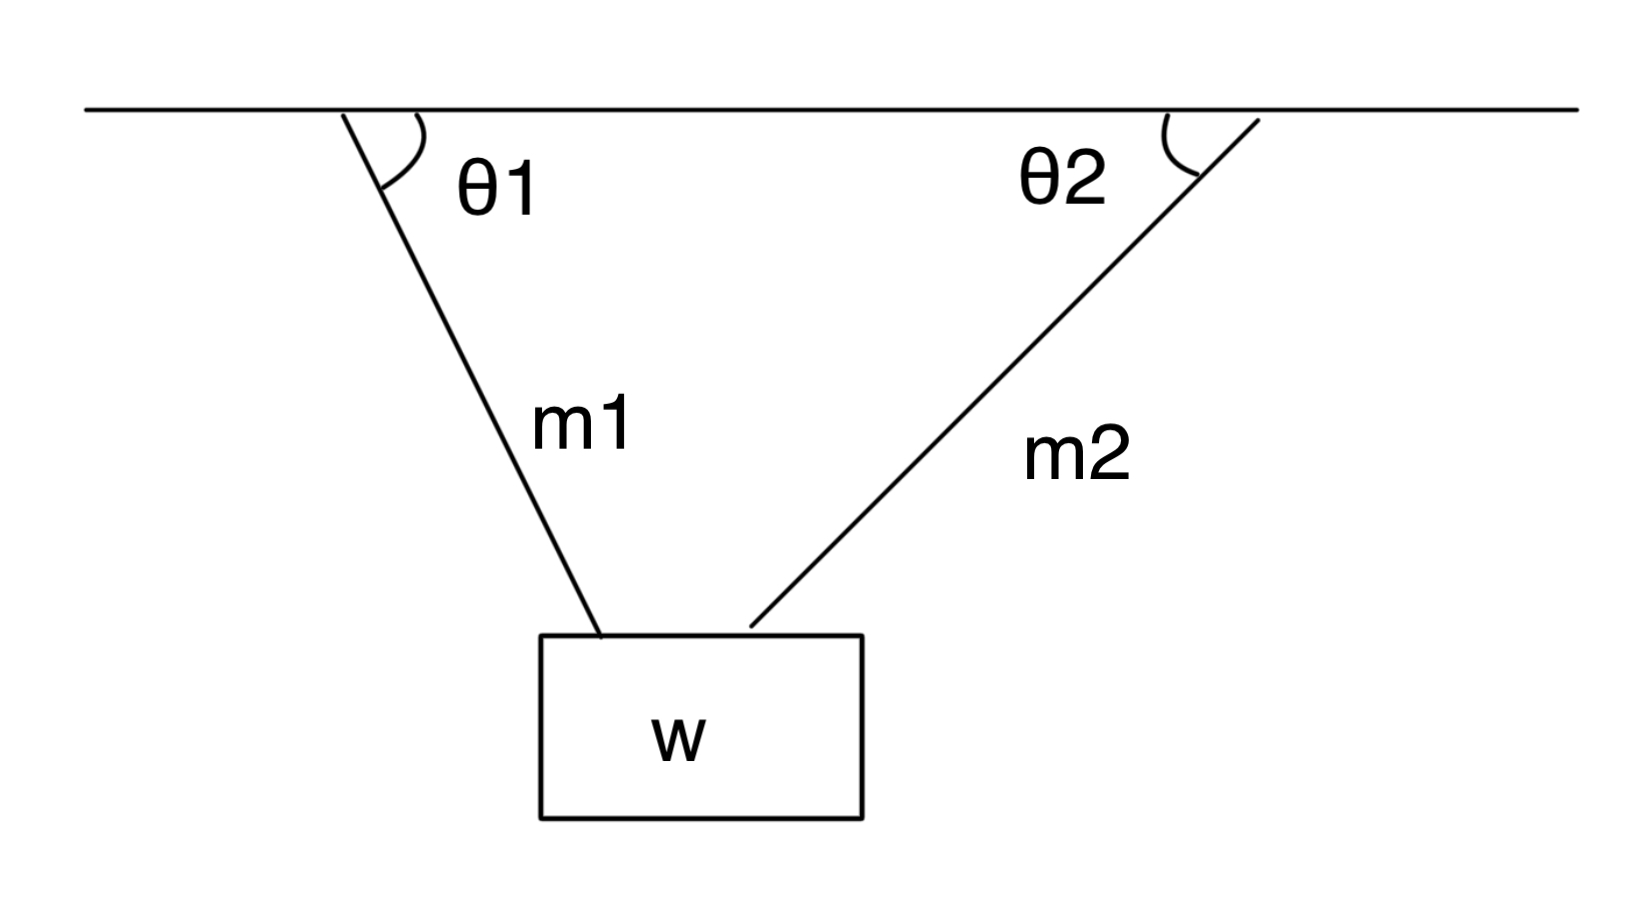
\includegraphics[width=6.5in]{./lab4diagram.png}
\captionof{figure}{\label{fig:setup}Experimental setup}
\end{center}
\subsection{The Testing Setup}
\label{sec:orgf10808b}

For the testing setup, we tied one end of line to a convenient location, a cross beam in the lab, and the other to a mass hanger. Then, we measured the length of the line with no weight \(l_1\). Then, we added some amount of weight, and remeasured the length of the line \(l_2\). We calculated the difference in the length of the line \(\Delta l = l_1 - l_2\). We repeated this process, adding more weight each time, until the line broke. The largest amount of mass that the line could hold without breaking is the maximum amount of weight that the line can hold. For the four pound line, we increased weight by 100g increments. For the eight pound line, we increased weight by 200g increments.

Additionally, we plotted \(\Delta l\) versus mass for our values to obtain a plot that shows the plastic and elastic regimes of the line.

\begin{center}
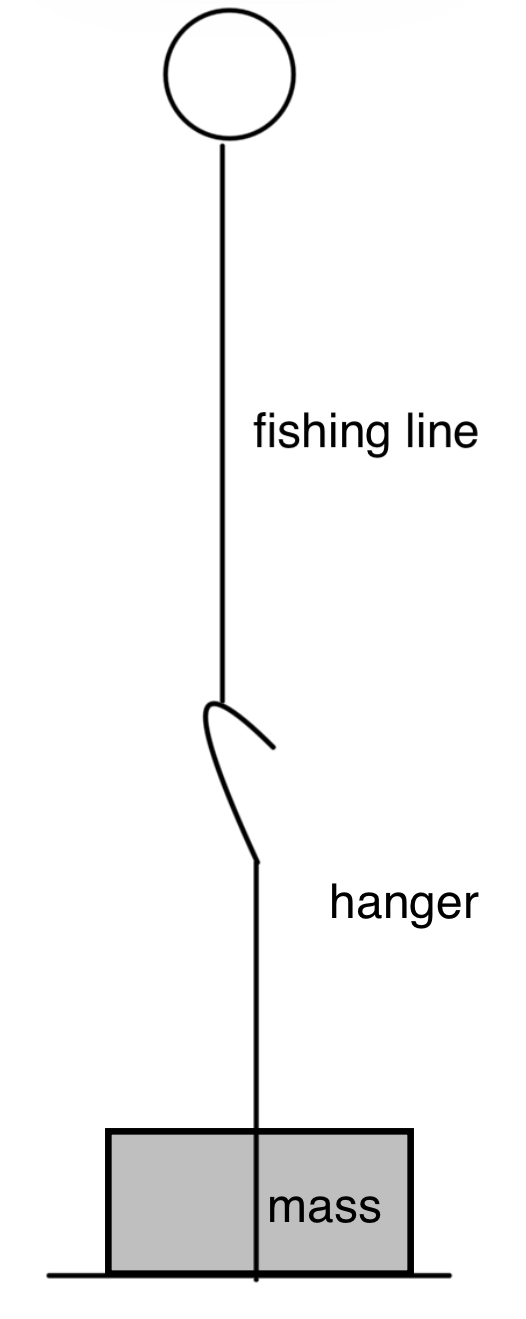
\includegraphics[height=5in]{./lab4hanger.png}
\captionof{figure}{\label{fig:test}Testing a line for its carrying capacity}
\end{center}
\section{Results}
\label{sec:orgcae8768}

Here is the result of testing the carrying capacity of the four pound line:

\begin{center}
\captionof{table}{\label{fig:four}Four pound line results}
\begin{tabular}{c|c|c|c}
Mass (g) & Length with mass (cm) & Length without mass (cm) & Change in length (cm)\\
\hline
200 & 54 & 51.3 & 2.7\\
300 & 55.2 & 51.3 & 3.9\\
400 & 55.9 & 51.5 & 4.4\\
500 & 56.6 & 51.9 & 4.7\\
600 & 57 & 52 & 5\\
700 & 57.7 & 52.2 & 5.5\\
800 & 58.3 & 52.4 & 5.9\\
900 & 58.6 & 52.4 & 6.2\\
1000 & 58.8 & 52.8 & 6\\
1100 & 59.4 & 52.8 & 6.6\\
1200 & 59.5 & 52.8 & 6.7\\
1300 & 59.8 & 53.2 & 6.6\\
1400 & 60.1 & 53.7 & 6.4\\
1500 & 60.6 & 53.5 & 7.1\\
1600 & 60.9 & 53.6 & 7.3\\
1700 & 61.5 & 53.7 & 7.8\\
1800 & 61.3 & 53.8 & 7.5\\
1900 & 62.3 & 54.2 & 8.1\\
2000 & 63 & 54.1 & 8.9\\
2100 & 63.6 & 54.8 & 8.8\\
2200 & 64.3 & 55.2 & 9.1\\
\end{tabular}
\end{center}

The line broke at 2300g. Here is the resulting graph of \(\Delta l\) versus mass:

\begin{center}
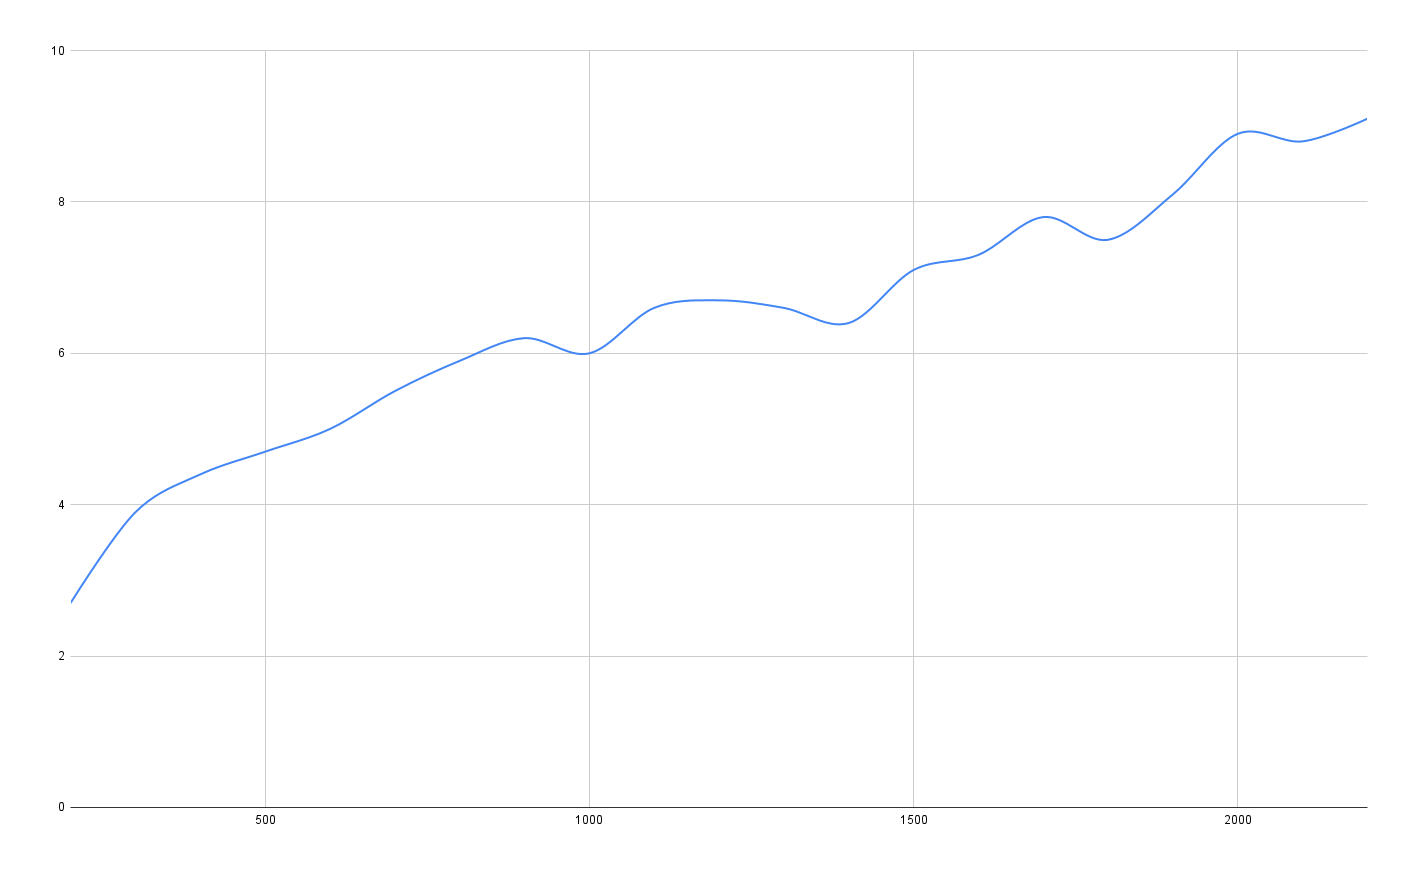
\includegraphics[width=6in]{./fourpoundchart.png}
\captionof{figure}{Four pound line \(\Delta l\) versus mass}
\end{center}

It appears as if the elastic domain is from [0, 1000] grams, with the plastic domain being from 1000 grams and on. In the elastic domain, \(\Delta l\) increases steadily. In the plastic domain, \(\Delta l\) plateaus, and then steadily increases. The transition between the plastic and elastic domains happens at the point where \(\Delta l\) plateaus.

Here is the result of testing the carrying capacity of the eight pound line:

\begin{table}[htbp]
\caption{\label{fig:eight}Eight pound line results}
\centering
\begin{tabular}{c|c|c|c}
Mass (g) & Length with mass (cm) & Length without mass (cm) & Change in length (cm)\\
\hline
400 & 63.9 & 63.5 & 0.4\\
500 & 69 & 63.6 & 5.4\\
550 & 69.4 & 63.6 & 5.8\\
600 & 69.7 & 63.7 & 6\\
650 & 69.8 & 63.8 & 6\\
700 & 69.9 & 63.9 & 6\\
800 & 70.5 & 65.1 & 5.4\\
900 & 71.2 & 65.1 & 6.1\\
1200 & 72 & 65 & 7\\
1450 & 72.5 & 64.5 & 8\\
1800 & 74 & 64.5 & 9.5\\
2000 & 74.5 & 65 & 9.5\\
\end{tabular}
\end{table}

The line broke unexpectedly at 2400g. Here is the resulting graph of \(\Delta l\) versus mass:

\begin{center}
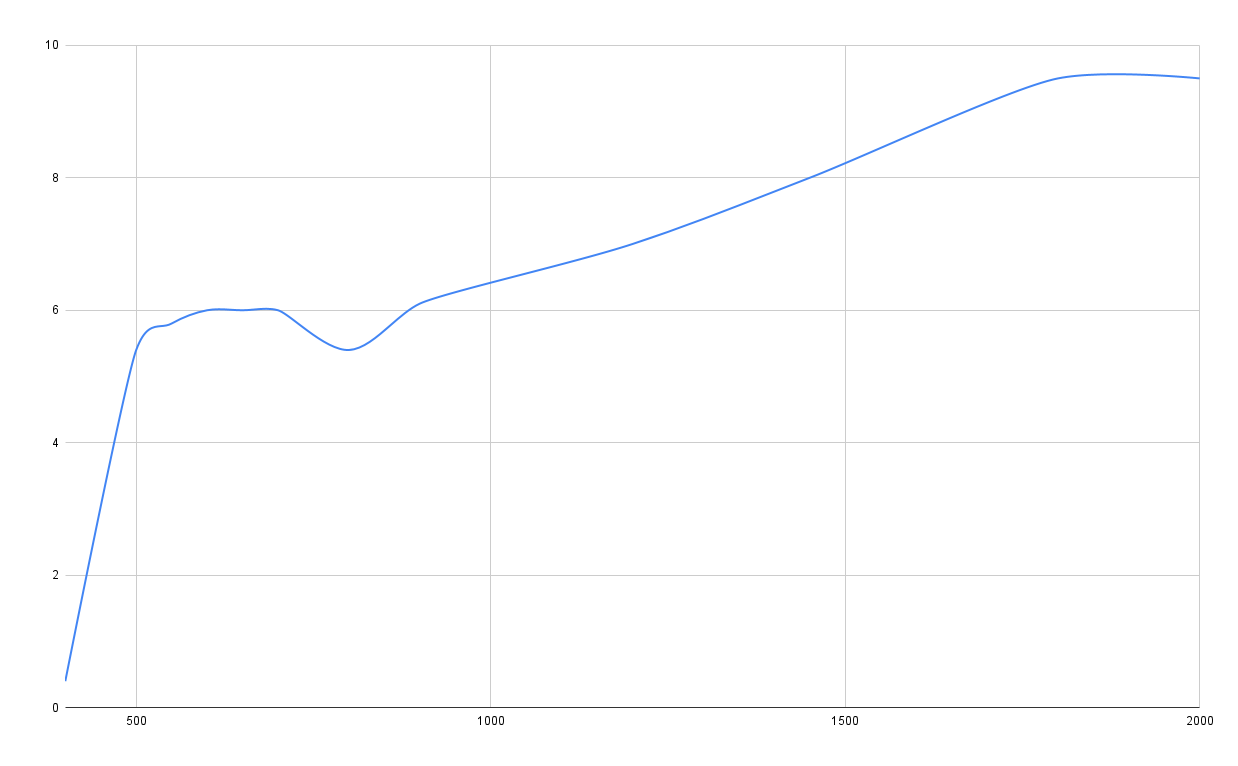
\includegraphics[width=6in]{./eightpoundchart.png}
\captionof{figure}{Eight pound line \(\Delta l\) versus mass}
\end{center}

It appears as if the elastic domain is from [0, 600] grams, with the plastic domain being from 600 grams and on. We observe the same dip.

Using Equations \ref{eq:tension} and \ref{eq:error}, we calculated that the four pound line would break with \(4.9\pm0.4\) kilograms of mass in the system, whereas the eight pound line would break with \(2.7\pm0.6\) kilograms of mass in the system. As such, we predicted the system would fail at 2.7 kilograms. When we put one kilogram of mass in the system, the system held fine. When we put three kilograms of mass in the system, one of the lines broke.
\section{Discussion}
\label{sec:orgce62dd9}

Our prediction was correct. The system failed when we exceeded the predicted threshold of 2.7 kilograms.

For obtaining the error, our professor decreed by magic that \(\sigma\)\textsubscript{\(\theta\)} would be \(2^{\circ}\). For \(\sigma_m\), we assumed that the true value for the maximum amount of tension the line could handle was between the largest stable value of \(m\) and the \(m\) that caused the line to break. As such, we set \(\sigma_m\) equal to the difference in that weight.

Wait. An eight pound line should be able to hold eight pounds of force. Ours failed at about five pounds of force.
\subsection{What happened to the eight pound line?}
\label{sec:org8785656}

Our line failed at a \emph{maximum} of 2400g. That is a maximum of 5.2 pounds of force. Theoretically, the line should have failed at a minimum of eight pounds, or 3.6 kilograms.

One possibility is our knot put too much stress on the fishing line, creating an abnormally weak area in the line. However, we used the same knot for all of our knots, so we would have observed this across both the four and eight pound lines. However, I do not believe this to be the case, since neither half hitches nor cinch knots put exorbitant stress on the line.

Another possibility is a manufacturing defect in the eight pound fishing line. This is possible, since (presumably) the eight pound line failed with a predicted \(m_{max}\) of \(2.7\pm0.6\) kilograms across both experiments.

There could be other factors having an effect on the result. Further experimentation is required.

Nonetheless, the eight pound line was consistent at which amount of tension in the line would break it.
\section{Sample Calculations}
\label{sec:org3ef35c3}

We used a spreadsheet for all of our calculations. To create the graphs, we selected the \texttt{mass} column as the y-axis, and the \texttt{delta l} column as the x-axis.

After getting the breakpoints for all of the lines, we put the relevant data into a convenient location. To determine \(m_1\), we used \texttt{=F25*(SIN(G27)+COS(G27)*TAN(I27))}, the spreadsheet version of Equation \ref{eq:tension}. Since we measured in grams, the result is in grams. Likewise, for \(m_2\) we used \texttt{=H25*(SIN(I27)+COS(I27)*TAN(G27))}. To determine \(\sigma_{m_1}^2\), we used the following equation:


\begin{verbatim}
=(sin(G27)+cos(G27)*tan(I27))^2*A32^2
    +(F25*(cos(G27)-sin(G27)*tan(I27)))^2*B32^2
    +(F25*(sin(G27)+cos(G27)*sec(I27)^2))^2*C32^2
\end{verbatim}

To determine \(\sigma_{m_1}\), we took the square root of that with \texttt{sqrt(A35)}.

Here are screenshots of the spreadsheets we used:

\begin{center}
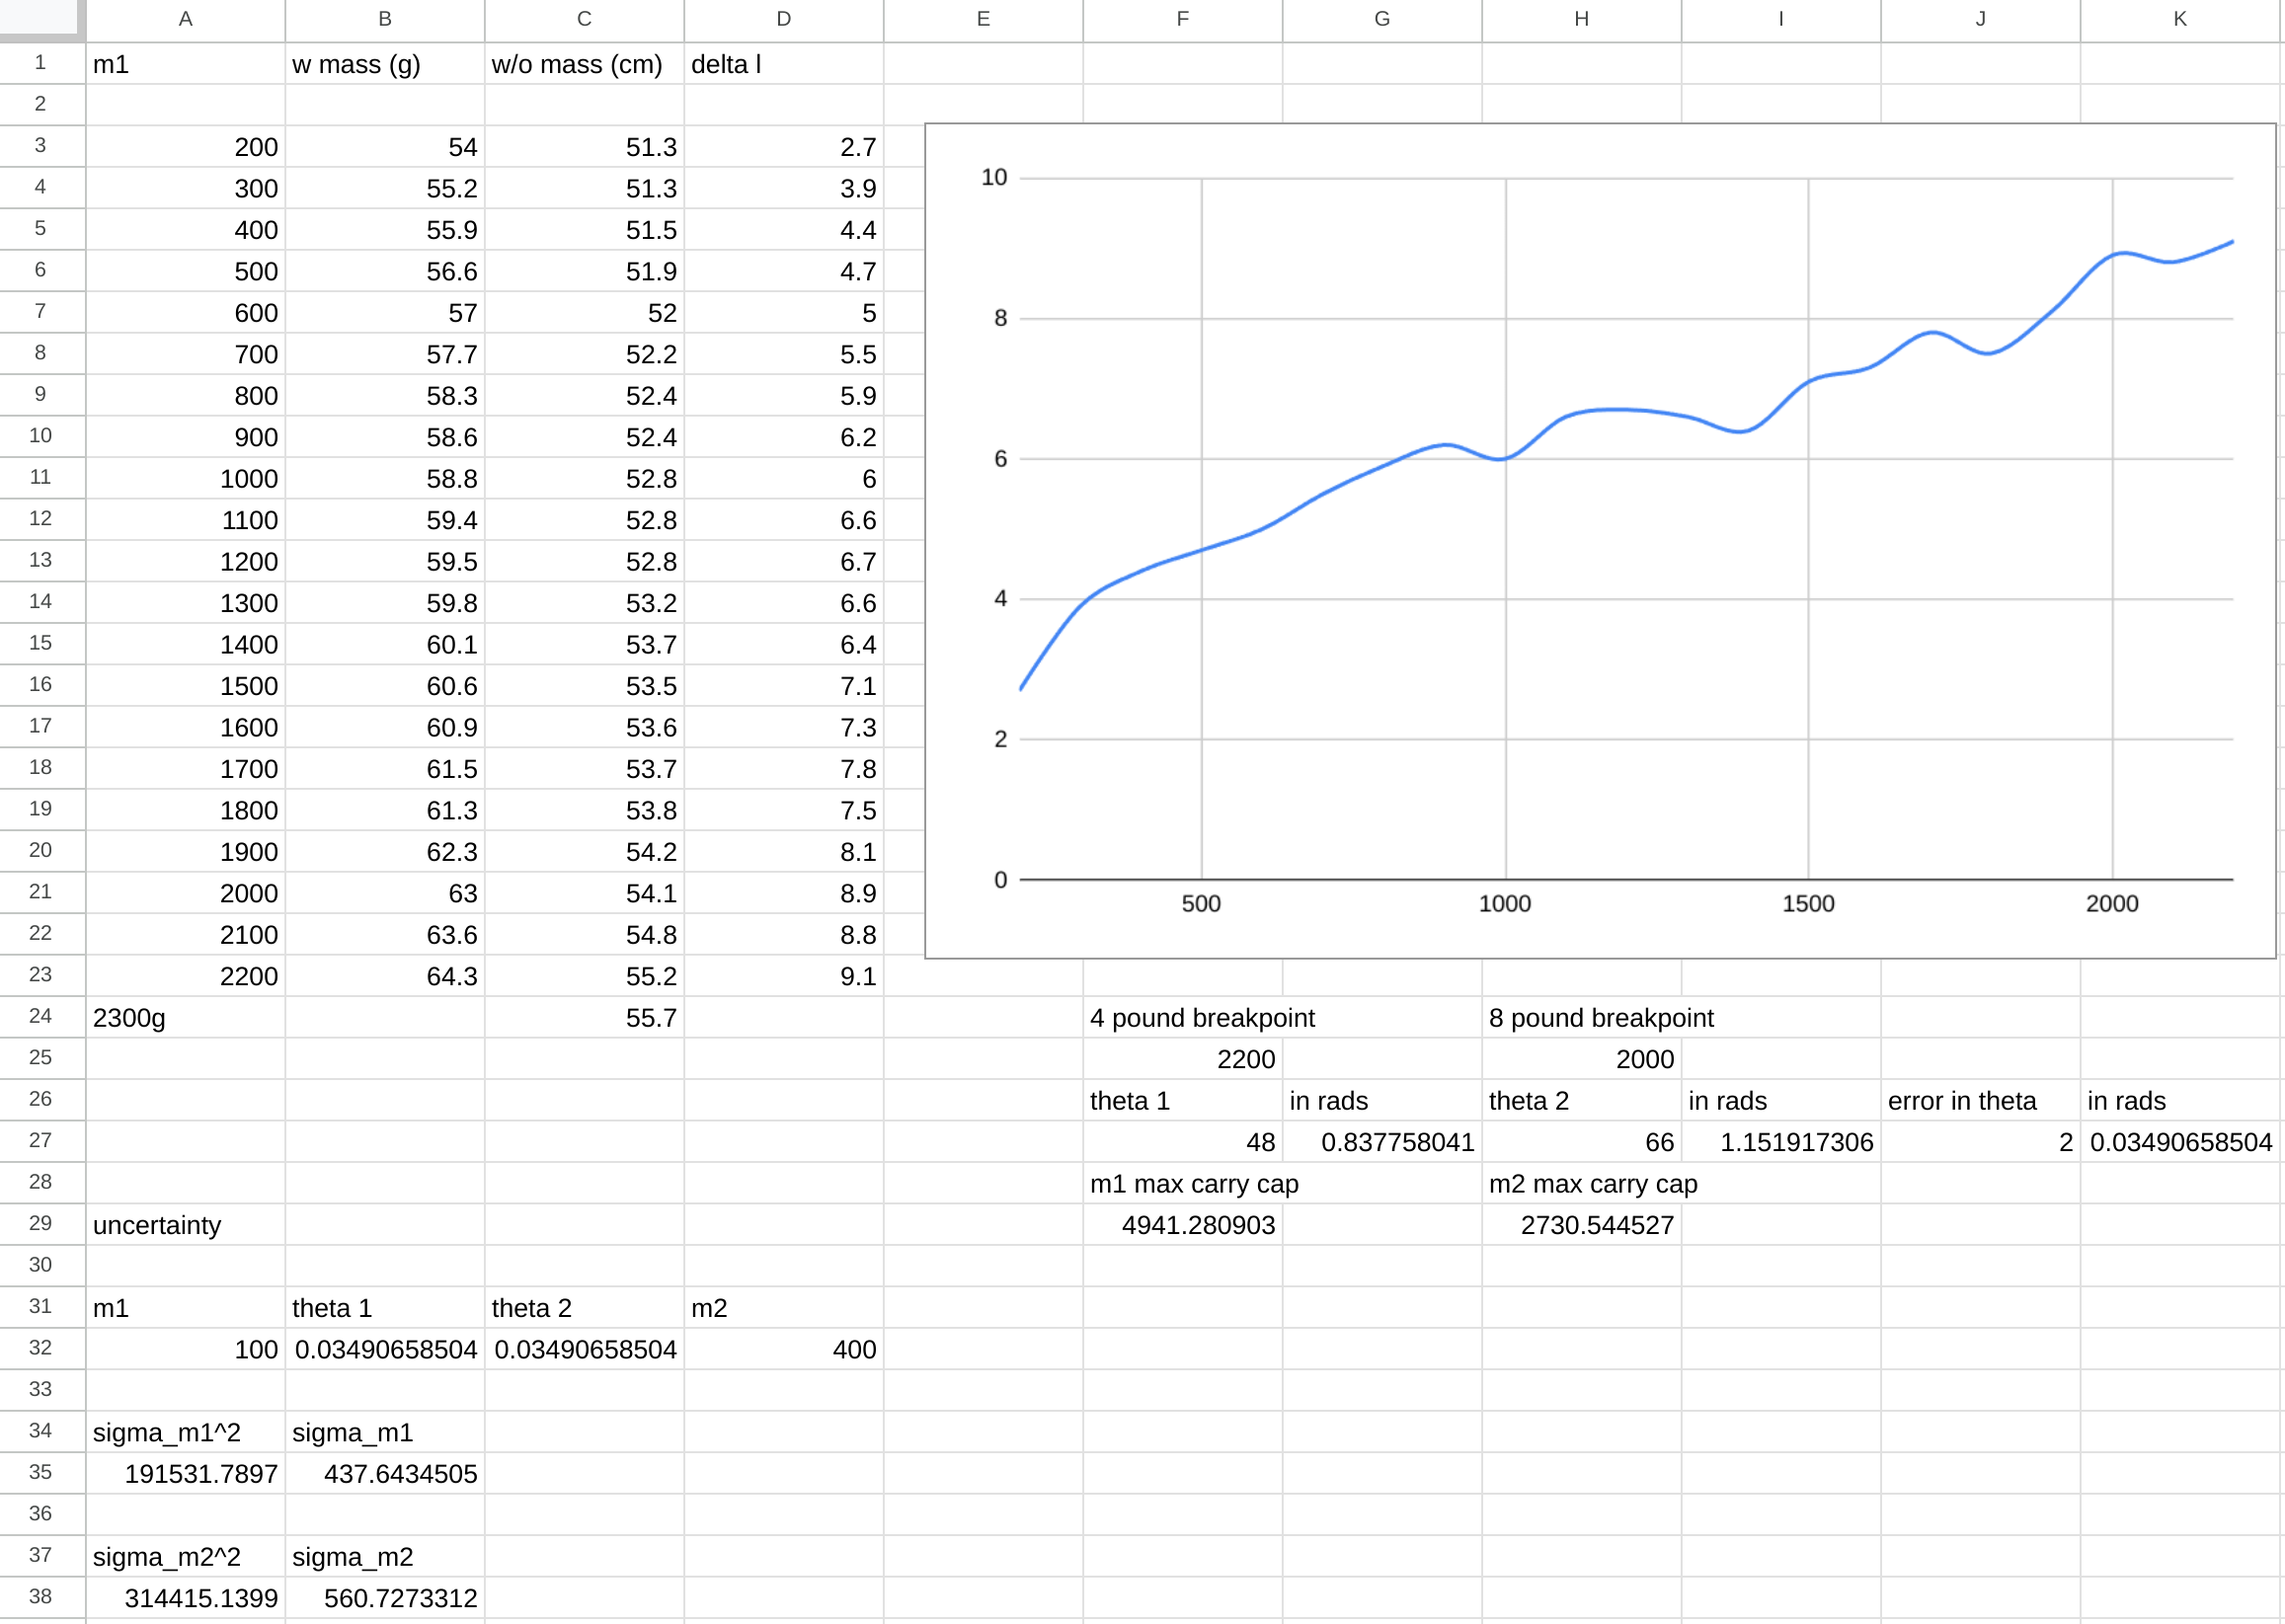
\includegraphics[width=6.5in]{./firstspread.png}
\end{center}

\begin{center}
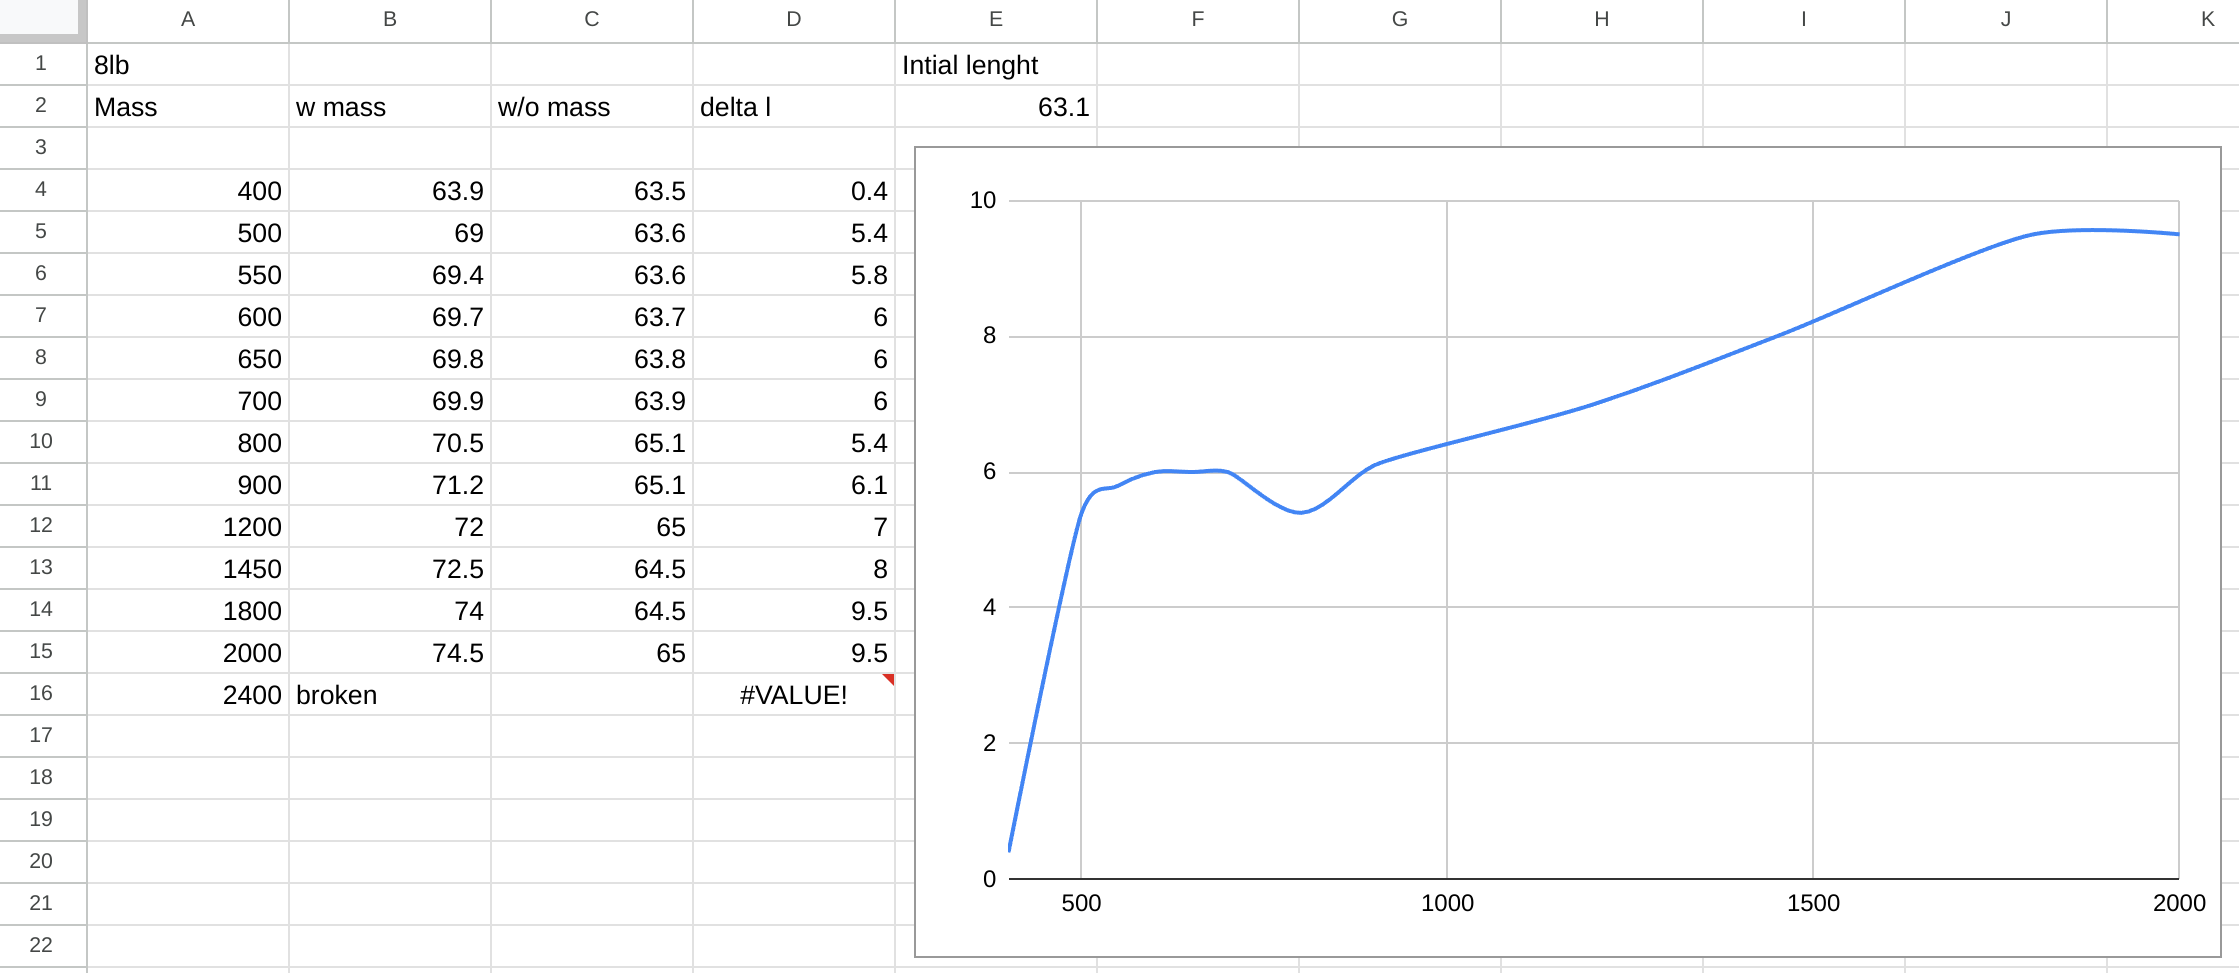
\includegraphics[width=6.5in]{./secondspread.png}
\end{center}
\end{document}
